% !TEX root=../main.tex

\section{Generating next step hints}
\label{sec:assistive}

This section introduces our \ASTOPHAT system.
%What do we wanna do?
The aim of \ASTOPHAT is to automatically provide next step hints.
When users follow these hints, they can be sure that they will reach the goal they described beforehand.
Users can, however, still decide to deviate from the given hints.

During the execution of \TOPHAT programs, users are presented with input fields, choices and continue buttons.
The way in which tasks progress and the resulting task value depend on these inputs.
At any point during execution, we would like to present users with all possible inputs that leads users to the goal they have selected.
These inputs are either concrete actions, like continue, pick the left task, pick the right task;
or a restricted set of values to be entered into an editor.
This set is restricted, since concrete values potentially influence the flow of the program.
To give a concrete example, the user should enter an integer, but this integer must be larger than zero to reach the end goal.

To come to these concrete actions and restricted values, we make use of symbolic execution.
In the next two sections, we briefly describe how symbolic execution for \TOPHAT works
and recap its symbolic semantics presented in earlier work~\cite{Naus2019}.
Thereafter, we show how to turn symbolic execution results into next step hints.
In \cref{sub:assistive-tax,sub:assistive-dining}, we study what these automatically generated hints look like for the examples from \cref{sec:examples}.

%% Our examples work in implementation
All examples have been tested in our implementation.
%% We have an implementation
We added \ASTOPHAT to our existing implementation of \STOPHAT, which is written in Haskell.\footnote{https://github.com/timjs/symbolic-tophat-haskell}
It uses the \ZTHREE \SMT solver under the hood.
%% It works like this
By defining the formal hints function directly on top of the symbolic execution semantics, % in \cref{fig:hints},
we can leverage the already existing symbolic execution for \STOPHAT in the practical implementation.


\subsection{Symbolic execution}
\label{sub:symbolic-execution}

A symbolic execution semantics~\cite{King1975,Boyer1975} aims to execute a program without knowing its input.
Instead, symbols are fed into the program.
During evaluation, the influence of values is recorded in the path condition.
The resulting symbolic value together with the path conditions can be used to prove properties of the program.

\begin{TASK}[
    float=ht,
    % numbers=right,
    caption={Ordering of tuple elements.},
    captionpos=b,
    label=lst:ordering]
  enter Int <&> enter Int >>= \<<x,y>>. if x > y then edit <<y, x>> else edit <<x, y>>
\end{TASK}

Consider the tiny example in \cref{lst:ordering}.
This program asks for two integer values.
After the user has entered this information, the function to the right of the step combinator makes sure the result will be an editor containing a pair,
where the second element is larger then the first.
When we run this program symbolically, we have to create fresh symbols to be entered in either of the two editors, say $s_0$ and $s_1$.
After entering both symbolic values and then normalising the task, there are two possible outcomes, namely
\begin{itemize}
  \item $\tuple{s_1,s_0}$, provided that the path condition $\phi_1 = s_0 > s_1$ holds; or
  \item $\tuple{s_0,s_1}$, with path condition $\phi_2 = \lnot (s_0 > s_1)$.
\end{itemize}

Now, the property that we want to prove for this program is that no matter what the input is, the second element should always be larger than the first.
We write this property as $\psi(\<a, b\>)= a \leq b$.
Looking at the two symbolic runs, we first need to verify that the symbolic runs are indeed viable.
This is done by checking that both $\phi_1$ and $\phi_2$ are satisfiable, written $\Sat(\phi_1)$ and $\Sat(\phi_2)$.
Symbolic runs with a path condition that is not satisfiable are discarded. 
Finally, we check that both path conditions conform to the goal property $\psi$, which is the case.
Therefore, we can conclude that the property holds.
When applying this technique to larger programs, it is a powerful tool to show that a program behaves as expected.


\subsection{Symbolic semantics}
\label{sub:symbolic-semantics}

To support symbolic execution in \TOPHAT, we extend our host language with symbols.
Also, we need to modify the semantics described in \cref{sub:semantics}, to accommodate symbolic execution.
The observation functions from \cref{sub:observations} are extended in a similar way.
These new semantic relations operate on expressions which may contain symbols.
Instead of stepping to one result, they lead to a set of possible results, accompanied with a path condition $\phi$.

\begin{table}[ht]
  \caption{}
  \label{tab:semantic-relations}
  \centering
  \begin{tabular}{l@{\Quad}L@{\Quad}L}
    \toprule
                  & \text{Concrete} & \text{Symbolic} \\
    \midrule
    Expressions   & e               & \tilde{e} \\
    Tasks         & t               & \tilde{t} \\
    States        & \sigma          & \tilde{\sigma} \\
    Inputs        & i               & \simi \\
    \midrule
    Evaluation    & \RelationE      & \RelationSE \\
    Normalisation & \RelationN      & \RelationSN \\
    Striding      & \RelationS      & \RelationSS \\
    Handling      & \RelationH      & \RelationSH \\
    Interacting   & \RelationI      & \RelationSI \\
    \bottomrule
  \end{tabular}
\end{table}

We denote entities containing symbols with an additional tilde,
and symbolic semantic relations with squiggly arrows instead of straight ones.
So $\tilde{t}$, $\tilde{\sigma}$, and $\simi$ are respectively tasks, states, and inputs containing symbols.
\Cref{tab:semantic-relations} gives an overview of entities in the concrete world,
and their symbolic counterparts.
\todo{Caption.}
%
Note that concrete expressions are a subset of symbolic expressions.
Therefore, symbolic semantic relations can be applied on concrete expressions,
as well as on symbolic expressions.

The symbolic interaction semantics ($\siminteract$) results in just one symbolic input.
In other words, it just looks ahead one symbolic interaction.
To be able to reason about an end goal after multiple symbolic interactions,
we introduce the notion of \emph{simulation}.
Informally, simulation performs multiple symbolic interactions after each other,
till the moment the rewritten task has an observable value.
I.e. if $n$ is the number of interactions needed to be done,
$\Value(t_i', \sigma_i')$ has a result for $i = n$ but is undefined for all $i < n$.
Next to that, we want to permit only viable executions.
This is enforced by validating the satisfiability ($\Sat$) of all path condition together.
More formally, simulating a task for multiple user inputs is defined as follows.

\begin{definition}[Simulation]
  \label{def:simulation}
  Let $t$ and $\sigma$ be a concrete task and concrete state.
  We define the simulation relation
  \begin{equation*}
    t,\sigma \simulate \overline{\tilde{v},\tilde{I},\Phi}
  \end{equation*}
  to be the set of results after performing symbolic interaction $n$ times:
  \begin{equation*}
      t,\sigma
        \siminteract \tilde{t}_1,\tilde{\sigma}_1,\simi_1,\phi_1
        \siminteract \cdots
        \siminteract \tilde{t}_n,\tilde{\sigma}_n,\simi_n,\phi_n
  \end{equation*}
  where:
  \begin{itemize}
    \item the $n$th task has a value: $\Value(\tilde{t}_n,\tilde{\sigma}_n) = \tilde{v}$;
    \item all tasks before do not have a value: $\Value(\tilde{t}_{i<n},\tilde{\sigma}_{i<n}) = \bot$;
    \item $\tilde{I} = \simi_1 \cdots \simi_n$ is the concatenation of all symbolic inputs generated along the way;
    \item $\Phi = \phi_1 \land \cdots \land \phi_n$, is the conjunction of all path conditions encountered.
  \end{itemize}
  Furthermore we require that:
  \begin{itemize}
    \item the resulting predicate is satisfiable: $\Sat(\Phi)$.
  \end{itemize}
\end{definition}

The simulation definition used in this paper differs from the one in previous work~\cite{Naus2019}.
Previously, infinite symbolic executions were filtered out by allowing two steps look-ahead in case of idempotent executions.
The definition above only allows finite executions by definition.

\todo{Use vending machine example to illustrate \STOPHAT?}


\subsection{Next step hints observation}
\label{sub:hints}

%% How do we do this?
As we have seen in \cref{def:simulation}, a symbolic task $\tilde{t}$ is considered done as soon as it has an observable value $\tilde{v}$.
In order to calculate next step hints, one needs to formulate a goal over this resulting value.
Only then, we can calculate next step hints for end users.

\begin{figure}
  \centering
  \usemacro{O-Hints}
  \caption{Definition of next step hint function.}
  \label{fig:hints}
\end{figure}

Hints are calculated by means of the $\Hints$ function listed in \cref{fig:hints}.
As input it receives a concrete task $t$ and concrete state $\sigma$ together with a goal predicate $g$.
The hints observation simulates $t$ starting in $\sigma$.
This results in a set of symbolic values $\tilde{v}$, together with a list of symbolic inputs $\tilde{I}$ and a condition $\Phi$ to reach this path.
We only want to use the symbolic executions that satisfy the goal $g$ when applied to $\tilde{v}$.
Since $\tilde{v}$ could contain symbols, it might be the case that $g(\tilde{v})$ is symbolic and would clash with the path condition $\Phi$.
Therefore, we require that the conjunction of the path condition with the goal is satisfiable ($\Sat(\Phi\land g(\tilde{v}))$).
From the executions that fulfill this requirement, we return the first symbolic input $\simi$ from the complete list of inputs $\simi\cdot\tilde{I}$,
together with the full condition that must hold ($\Phi\land g(\tilde{v})$).
The resulting set contains pairs of symbolic inputs guarded by this condition.

To get a better understanding how $\Hints$ works,
we study it more concretely in the next subsections.
\Cref{sub:assistive-tax} demonstrates on the basis of the tax example listed in \cref{sec:tax} how the results of the symbolic execution are used to construct automatic next step hints.
\Cref{sub:assistive-dining} shows how hints can be generated during the execution of the example \TOPHAT program listed in \cref{sec:dining}.


\subsection{Tax subsidy request}
\label{sub:assistive-tax}

%recall
Recall the Tax example program in \TOPHAT from \cref{sec:tax},
which models the application for a solar panel tax refund.
The user enters the invoice date and invoice amount, the installation company confirms, and finally the tax officer either approves or denies the request.

\begin{table}[ht]
  \caption{The results of simulating the program from \cref{lst:tax}.}
  \label{table:tax}
  \centering
  \begin{tabular}{LLL}
    \toprule
    \text{Symbolic value ($\tilde{v}$)} & \text{Symbolic input ($\tilde{I}$)} & \text{Path condition ($\Phi$)} \\
    \midrule
    \tuple{\min(600, s_{\id{a}}/10),  \True, \True, s_{\id{i}}, \Today} & \First \First s_{\id{a}} \cdot \First \Second s_{\id{i}} \cdot \Second \Left \cdot \Second & (\Today-s_{\id{i}}) < \OneYear \\
    \tuple{\min(600, s_{\id{a}}/10),  \True, \True, s_{\id{i}}, \Today} & \First \Second s_{\id{i}} \cdot \First \First s_{\id{a}} \cdot \Second \Left \cdot \Second & (\Today-s_{\id{i}}) < \OneYear \\
    \tuple{\min(600, s_{\id{a}}/10),  \True, \True, s_{\id{i}}, \Today} & \Second \Left \cdot \First \First s_{\id{a}} \cdot \First \Second s_{\id{i}} \cdot \Second & (\Today-s_{\id{i}}) < \OneYear \\
    \tuple{\min(600, s_{\id{a}}/10),  \True, \True, s_{\id{i}}, \Today} & \Second \Left \cdot \First \Second s_{\id{i}} \cdot \First \First s_{\id{a}} \cdot \Second & (\Today-s_{\id{i}}) < \OneYear \\
    \tuple{\min(600, s_{\id{a}}/10),  \True, \True, s_{\id{i}}, \Today} & \First \Second s_{\id{i}} \cdot \Second \Left \cdot \First \First s_{\id{a}} \cdot \Second & (\Today-s_{\id{i}}) < \OneYear \\
    \tuple{\min(600, s_{\id{a}}/10),  \True, \True, s_{\id{i}}, \Today} & \First \First s_{\id{a}} \cdot \Second \Left \cdot \First \Second s_{\id{i}} \cdot \Second & (\Today-s_{\id{i}}) < \OneYear \\
    \midrule
    \tuple{                       0,  \False, \True, s_{\id{i}}, \Today} & \First \First s_{\id{a}} \cdot \First \Second s_{\id{i}} \cdot \Second \Left \cdot \First  & \True \\
    \tuple{                       0,  \False, \True, s_{\id{i}}, \Today} & \First \Second s_{\id{i}} \cdot \First \First s_{\id{a}} \cdot \Second \Left \cdot \First  & \True \\
    \tuple{                       0,  \False, \True, s_{\id{i}}, \Today} & \Second \Left \cdot \First \First s_{\id{a}} \cdot \First \Second s_{\id{i}} \cdot \First  & \True \\
    \tuple{                       0,  \False, \True, s_{\id{i}}, \Today} & \Second \Left \cdot \First \Second s_{\id{i}} \cdot \First \First s_{\id{a}} \cdot \First  & \True \\
    \tuple{                       0,  \False, \True, s_{\id{i}}, \Today} & \First \Second s_{\id{i}} \cdot \Second \Left \cdot \First \First s_{\id{a}} \cdot \First  & \True \\
    \tuple{                       0,  \False, \True, s_{\id{i}}, \Today} & \First \First s_{\id{a}} \cdot \Second \Left \cdot \First \Second s_{\id{i}} \cdot \First  & \True \\
    \tuple{                       0,  \False,\False, s_{\id{i}}, \Today} & \First \First s_{\id{a}} \cdot \First \Second s_{\id{i}} \cdot \Second \cdot \First  & \True \\
    \tuple{                       0,  \False,\False, s_{\id{i}}, \Today} & \First \Second s_{\id{i}} \cdot \First \First s_{\id{a}} \cdot \Second \cdot \First  & \True \\
    \tuple{                       0,  \False,\False, s_{\id{i}}, \Today} & \Second \Second \cdot\First \First s_{\id{a}} \cdot \First \Second s_{\id{i}} \cdot \First  & \True \\
    \tuple{                       0,  \False,\False, s_{\id{i}}, \Today} & \Second \cdot \First \Second s_{\id{i}} \cdot \First \First s_{\id{a}} \cdot \First  & \True \\
    \tuple{                       0,  \False,\False, s_{\id{i}}, \Today} & \First \Second s_{\id{i}} \cdot \Second \cdot \First \First s_{\id{a}} \cdot \First  & \True \\
    \tuple{                       0,  \False,\False, s_{\id{i}}, \Today} & \First \First s_{\id{a}} \cdot \Second \cdot \First \Second s_{\id{i}} \cdot \First  & \True \\
    \bottomrule
  \end{tabular}
\end{table}

In this section, we will demonstrate what symbolic execution looks like for this example, and how we generate next step hints from the symbolic execution results.
First, we call the simulate function $\simulate$ on the program, with an empty state.
The resulting set of symbolic executions is listed in \cref{table:tax}.
Each line represents one symbolic execution.
In the first column, the resulting symbolic value $\tilde{v}$ is listed.
The second column lists the symbolic input $\tilde{I}$ that was produced to arrive at that value, followed by the path condition $\Phi$ in the third column.
The symbolic values that are produced are $s_i$ for the invoice date and $s_a$ for the invoice amount.

The definition of $\Hints$ describes how these results should be used in order to calculate next step hints.
First of all, we need a goal $g$ to select the symbolic runs that we are interested in.
The most straight forward goal would be that we want to end up in a situation where we get a subsidy amount larger than zero.
This goal can be formulated as $g(\tuple{v,\_,\_,\_,\_}) = v > 0$.

The first six symbolic runs listed in \cref{table:tax} fulfill this goal condition.
From those runs, we then take the first symbolic input, together with the path condition conjugated with the goal.
After removing duplicates and redundant information, the result of $\Hints$ is as follows.
\begin{block}
  \begin{tabular}{LCL}
    \tuple{\First \First s_{\id{a}}  &, & \min(600, s_{\id{a}}/10) > 0}  \\
    \tuple{\First \Second s_{\id{i}} &, & (\Today-s_{\id{i}}) < \OneYear} \\
    \tuple{\Second \Left             &, & \True} 
  \end{tabular}
\end{block}
This means that, at this stage, users have three possible options.\footnote{
  Note that the first branch, entering an amount, is denoted by $\First \First$;
  the second branch, entering the invoice date, is denoted by $\First \Second$;
  and the third branch, making a left/right choice, is denoted by $\Second$.
}
\begin{enumerate}
  \item The applicant may enter an amount $s_\id{a}$ for which $\min(600, s_{\id{a}}/10) > 0$ should hold.
  \item The applicant may enter an invoice date $s_\id{i}$ for which $(\Today-s_{\id{i}}) < \OneYear$ should hold.
  \item The company should take the left choice ($\Left$) to confirm they installed the solar panels. 
\end{enumerate}


\subsection{Dining Computer Scientists}
\label{sub:assistive-dining}

%% Recall
Recall the example program Dining Computer Scientists from \cref{sec:dining}.
Three computer scientist sit at a table and have to coordinate how to their meals.
%% What hints do we want to give?
We want to calculate all possible next steps that lead to the goal.
The goal in this example is for all computer scientists to finish their meal.
%% Write the goal
In terms of the resulting task value, this means that we want to reach the value "Full bellies".
Witten as a predicate, we get $g(v) = v \equiv \text{"Full bellies"}$.

%% What does the result of H look like?
Let us assume that both Grace Hopper and Ada Lovelace have already picked up the forks to their left ($\lbl{fork1}$ and $\lbl{fork2}$ respectively).
We then find ourselves in the situation shown in \cref{fig:dining-middle}.
\todo{REPLACE THIS IMAGE!}

\begin{figure}[t]
  \centering
  \begin{minipage}[r]{0.65\textwidth}
    \noindent Current program:
    \begin{TASK}[xleftmargin=1.5em]
  ( scientist "Alan Turing" fork0 fork1
      <&>
    <<>> >>? \ _. if !fork2 then(edit fork1 := True) else fail
      <&>
    <<>> >>? \ _. if !fork0 then(edit fork2 := True) else fail
  ) >>= \ _ . edit "Full bellies"
    \end{TASK}
    \vspace*{\medskipamount}
    Current state:\\
    \hspace*{1.5em} $\sigma = \set{\text{fork0}\mapsto \True, \text{fork1}\mapsto \False,\text{fork2}\mapsto \False}$
  \end{minipage}
  \begin{minipage}[r]{0.3\textwidth}
    \tikzset{every picture/.style={line width=0.75pt}} %set default line width to 0.75pt
    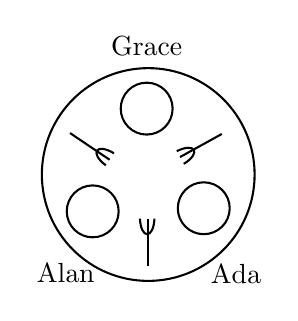
\begin{tikzpicture}[x=0.75pt,y=0.75pt,yscale=-0.5,xscale=0.5]
      %uncomment if require: \path (0,300); %set diagram left start at 0, and has height of 300
      %Shape: Circle [id:dp8519268538531043]
      \draw   (229,147.5) .. controls (229,90.89) and (274.89,45) .. (331.5,45) .. controls (388.11,45) and (434,90.89) .. (434,147.5) .. controls (434,204.11) and (388.11,250) .. (331.5,250) .. controls (274.89,250) and (229,204.11) .. (229,147.5) -- cycle ;
      %Shape: Circle [id:dp8204933417548707]
      \draw   (305,84) .. controls (305,70.19) and (316.19,59) .. (330,59) .. controls (343.81,59) and (355,70.19) .. (355,84) .. controls (355,97.81) and (343.81,109) .. (330,109) .. controls (316.19,109) and (305,97.81) .. (305,84) -- cycle ;
      %Shape: Circle [id:dp7478076126793654]
      \draw   (360,180) .. controls (360,166.19) and (371.19,155) .. (385,155) .. controls (398.81,155) and (410,166.19) .. (410,180) .. controls (410,193.81) and (398.81,205) .. (385,205) .. controls (371.19,205) and (360,193.81) .. (360,180) -- cycle ;
      %Shape: Circle [id:dp3120260710082954]
      \draw   (253,183) .. controls (253,169.19) and (264.19,158) .. (278,158) .. controls (291.81,158) and (303,169.19) .. (303,183) .. controls (303,196.81) and (291.81,208) .. (278,208) .. controls (264.19,208) and (253,196.81) .. (253,183) -- cycle ;
      %Straight Lines [id:da6820891014633774]
      \draw    (331,190) -- (331,236) ;
      %Curve Lines [id:da1548185264621137]
      \draw    (323.5,190) .. controls (324.5,210) and (336.5,210) .. (337.5,190) ;
      %Straight Lines [id:da4306446303925887]
      \draw    (294.3,133.27) -- (256.15,107.56) ;
      %Curve Lines [id:da9253738091345234]
      \draw    (298.49,127.05) .. controls (281.34,116.7) and (274.64,126.65) .. (290.66,138.66) ;
      %Straight Lines [id:da7927760692654279]
      \draw    (362.12,130.68) -- (402.39,108.44) ;
      %Curve Lines [id:da6105283277592903]
      \draw    (365.75,137.25) .. controls (382.77,126.7) and (376.97,116.2) .. (358.98,124.99) ;
      % Text Node
      \draw (252,242) node  [align=left] {Alan};
      % Text Node
      \draw (330,24) node  [align=left] {Grace};
      % Text Node
      \draw (416,243) node  [align=left] {Ada};
    \end{tikzpicture}
  \end{minipage}
  \caption{Task, state and visual representation after two interactions}
  \label{fig:dining-middle}
\end{figure}

Calling $\Hints(t,\sigma,g)$ will result in just one hint, namely
\begin{equation*}
  \tuple{\Second\Second\Continue,\True}.
\end{equation*}
This means that the only step towards goal $g$ is for the third scientist,\footnote{
  The third branch is denoted by $\Second\Second$.
  $\Continue$ means pushing the continue button.
}
which is Ada Lovelace, to pick up the right fork.
Although it is also possible for Alan Turing to pick up the fork to his left,
this step is not a valid hint and performing this action will result in deadlock.

